\chapter{Opis problemu układania planu zajęć}
\textit{Tomasz Dziopa}
\paragraph{}Układanie planu zajęć można sformułować jako problem przydzielenia zdarzeń do przedziałów czasowych i zasobów, w taki sposób, żeby nie naruszyć odpowiednio skonstruowanych ograniczeń. Ograniczenia można podzielić na:
\begin{itemize}
\item ,,twarde'' - naruszenie ich powoduje, że utworzony plan zajęć jest niepoprawny,
\item ,,miękkie'' - naruszenia ich wyznaczają jakość utworzonego poprawnego planu zajęć. Im więcej naruszeń, tym jakość planu jest niższa.
\end{itemize}
\paragraph{}W przypadku problemu układania planu zajęć na uczelni problem możemy sprowadzić do następującej postaci:
\begin{itemize}
\item zdarzeniami będą powtarzające się zajęcia - wykłady, laboratoria, lekcje
\item zasobami będą sale, w których są prowadzone zajęcia i wykładowcy
\item ograniczenia twarde najczęściej uwzględniają:
	\begin{itemize}
	\item zajęcia dla jednej klasy nie mogą odbywać się w tym samym czasie,
	\item wykładowca nie może prowadzić równocześnie dwóch różnych zajęć,
	\item w jednej sali mogą odbywać się tylko jedne zajęcia,
	\item niektóre zajęcia muszą odbywać się w sali przystosowanej do specyfiki zajęć 
	\end{itemize}
\item ograniczenia miękkie definiuje się odrębnie dla placówek zależnie od ich priorytetów
\end{itemize}



%Problem układania planu zajęć jest niezwykle ważnym problemem. Jest obecny w wielu dziedzinach, gdyż przy niewielkich modyfikacjach można przenieść go na problem ustalania rozkładów jazdy, czy planowania grafiku pracowników, gdzie znalezienie lepszego rozwiązania prowadzi do oszczędności czasu i zasobów. 
\section{Klasyfikacja problemu}
\subsection{Problem NP-zupełny}
\paragraph{}Problem układania planu zajęć jest klasyfikowany jako NP-zupełny, co można w łatwy sposób udowodnić poprzez redukcję problemu k-kolorowania wierzchołkowego grafu $G(V, E)$, gdzie $V$ zawiera zdarzenia, a $E$ konflikty między nimi, do decyzyjnej wersji problemu układania planu zajęć (czy da się skonstruować plan zajęć obejmujący $k$ przedziałów czasowych) 
\paragraph{}Problem k-kolorowania wierzchołkowego to problem decyzyjny, który polega na odpowiedzi na pytanie, czy dany graf da się pokolorować wierzchołkowo na dokładnie $k$ kolorów. Przypomnijmy, że w każdym poprawnym pokolorowaniu każde dwa wierzchołki połączone ze sobą krawędzią muszą mieć przyporządkowane różne kolory. W grafie $G(V,E)$ krawędziami połączone są zdarzenia, które nie mogą odbywać się w tym samym czasie. Jeżeli przyjmiemy, że kolorom w pokolorowaniu odpowiadają poszczególne przedziały czasowe otrzymujemy redukcję w czasie wielomianowym ze względu na liczbę wierzchołków i krawędzi do problemu k-kolorowania wierzchołkowego grafu. Bardziej formalny dowód na tą redukcję, jak i inne redukcje z innych problemów NP-zupełnych zawiera \cite{npcomplete}.


\section{Przegląd algorytmów}
\subsection{Metaheurystyki}
\paragraph{}Problem układania planu zajęć jest NP-zupełny, więc nie istnieje deterministyczny algorytm, który zwracałby dokładny wynik w czasie wielomianowym. Konieczne jest więc zastosowanie \textbf{metaheurystyk} - niedeterministycznych algorytmów, które wspomagają przeszukiwanie przestrzeni rozwiązań, w celu znalezienia najlepszego rozwiązania. Metaheurystyki często bazują na obserwacjach różnych procesów zachodzących w naturze. Znane są zastosowania różnego rodzaju metaheurystyk do rozwiązania naszego problemu.
\subsubsection{Algorytm genetyczny}
\paragraph{} Być może najbardziej popularne i uniwersalne rozwiązanie. Proces optymalizacji rozwiązania odwzorowuje sposób ewolucji genetycznej osobników przystosowujących się do środowiska, w którym przebywają. Swoje odwzorowanie mają zatem metody selekcji lepiej przystosowanych osobników, którzy dożyją następnego pokolenia, operacja krzyżowania osobników w celu stworzenia potomstwa czy też mutacja wprowadzająca drobne zmiany w materiale genetycznym. Algorytm iteracyjne polepsza swoje rozwiązanie coraz dokładniej przeszukując przestrzeń możliwych rozwiązań. Czynnik losowy odgrywa dużą rolę w wymienionych wcześniej procesach, co nie gwarantuje bardzo skutecznych rezultatów.
\subsubsection{Algorytm wyszukiwania harmonicznego}
Jedno z najnowszych rozwiązań (powstałe w 2001 roku). Naśladuje proces poszukiwania harmonii przez grających razem muzyków, której jakość jest miarą rozwiązania. Przechowując w pamięci najlepsze dotychczasowe współbrzmienia oraz tworząc nowe (losowe) wysokości odgrywanych dźwięków, muzycy poprawiają wzajemną harmonię. Rozwiązanie to początkowo zebrało wiele pozytywnych recenzji i zakładano, że może wnieść wiele skutecznych rozwiązań w dziedzinie problemów optymalizacyjnych, lecz nadzieje te zostały porzucone ze względu na duże podobieństwa do pozostałych algorytmów ewolucyjnych.
\subsubsection{Algorytm optymalizacji rojem cząsteczek}
Metoda ta stara się naśladować zachowania występujące w przyrodzie. Jest to technika ewolucyjna wzorowana na sposobie poruszania się i inteligencji roju owadów poszukującego optymalnego miejsca do pożywienia się. Dokładniejszy opis algorytmu znajduje się w punkcie 4.2.

\subsubsection{Algorytm symulowanego wyżarzania}
\paragraph{} Metoda przeszukiwania iteracyjnego zainspirowana procesem wyżarzania w przemyśle metalowym. Przechowujemy specjalną zmienną, która symuluje malejącą ,,temperaturę'' otoczenia. W każdej iteracji przeglądamy sąsiadów i z prawdopodobieństwem proporcjonalnym do ,,temperatury'' akceptujemy rozwiązanie gorsze od aktualnego.


\subsubsection{Algorytm Tabu Search}
\paragraph{} Metoda iteracyjnego przeszukiwania najlepszego rozwiązania, która bazuje na liście tabu - liście ruchów zabronionych, których nie można wykonać przez określoną liczbę iteracji. Dokładny opis algorytmu znajduje się w punkcie 4.1.3.

\subsection{Hiperheurystyki}
\paragraph{}Nieco innym podejściem do rozwiązania problemu układania planu zajęć jest zastosowanie hiperheurystyki. \textbf{Hiperheurystyka} to algorytm, który ma za zadanie odnalezienie najlepszej metaheurystyki mającej na celu znaleźć optymalne rozwiązanie. Przykładem hiperheurystyki może być algorytm Adaptive Tabu Search, opisany szerzej w punkcie 4.1, gdzie metaheurystykami niskiego poziomu są procedury Tabu Search dla dwóch struktur sąsiedztwa, a metaheurystyką jest iteracyjne przeszukiwanie lokalne, które steruje głębokością procedury Tabu Search i wprowadza operator zaburzeń rozwiązania.
\paragraph{}Innym przykładem hiperheurystyki jest algorytm opisany w \cite{gbhh}. Autorzy jako metaheurystyki niskiego poziomu wybrali 5 różnych kolejności, w których można rozpatrywać wierzchołki grafu kursów i konfliktów między nimi. Metaheurystyka wysokiego poziomu - w tym przypadku Tabu Search, gdzie lista Tabu przechowuje kombinacje dwuelementowe metaheurystyk niskiego poziomu - wybiera dwie metaheurystyki, które nie występują na liście Tabu, przyporządkowywuje według nich kolejne kursy i porównuje wynik z najlepszym.

\subsection{Algorytmy \textit{state-of-the-art}}

\paragraph{} Inną grupą algorytmów, na które można się natknąć w literaturze są algorytmy tzw. \textit{state-of-the-art} - wielofazowe algorytmy, które kolejnych fazach wykonują po kilka różnych metaheurystyk. Przykładem takiego algorytmu jest algorytm, który wygrał konkurs ITC w 2003 roku, opisany w \cite{kostuch}.


\section{Przegląd powstałych systemów}



\subsection{aSc TimeTables}
Rozbudowane komercyjne narzędzie, które umożliwia automatyczne wygenerowanie planu zajęć na podstawie zebranych wymagań. Posiada bardzo zaawansowane możliwości edycji wygenerowania planu, wprowadzania zastępstw nauczycieli i wizualizacji. Możliwości sterowania generowaniem są ograniczone - można ustalić czas generowania (krótki - długi - bardzo długi) i stopień spełniania warunków. Program jest adresowany do dyrektorów i osób zarządzających planami lekcji, jego obsługa jest bardzo prosta. Wadą jest scentralizowane wprowadzanie ograniczeń, nieestetyczny interfejs i cena 
(od 499 USD za wersję podstawową, do 3995 USD za wersję z rozszerzonym wsparciem i generowaniem planów dla poszczególnych uczniów)
\begin{figure}[H]
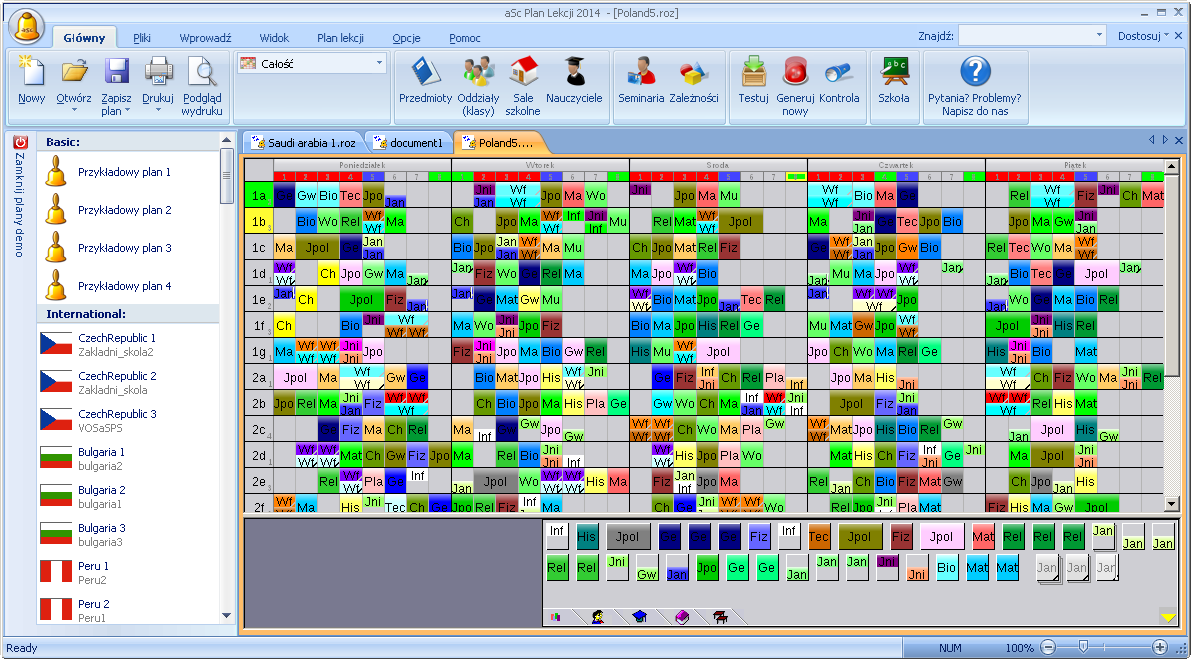
\includegraphics[width=15cm]{img/asc2.png}
\caption{Zrzut ekranu z programu aSc. Przy przenoszeniu zajęć konfliktujące okresy podświetlają się na czerwono}
\end{figure}

\subsection{Mimosa}
Komercyjny program, który umożliwia wprowadzanie ograniczeń, automatyczne generowanie planu zajęć i optymalizowanie już istniejącego planu. Interfejs aplikacji jest nieczytelny i chaotyczny, cały program sprawia wrażenie przestarzałego. Nie można sterować procesem generowania, który jest realizowany w bardzo szybki sposób, jednak dla przykładowych danych nie przydziela wszystkich zajęć, pomimo tego, że jest to możliwe. Aplikacja jest uniwersalna, można dostosowywać problem do własnych potrzeb, jednak bez uprzedniego przeszkolenia jest to bardzo trudne. Najtańsza licencja na jedno stanowisko kosztuje 500 euro.
\begin{figure}[H]
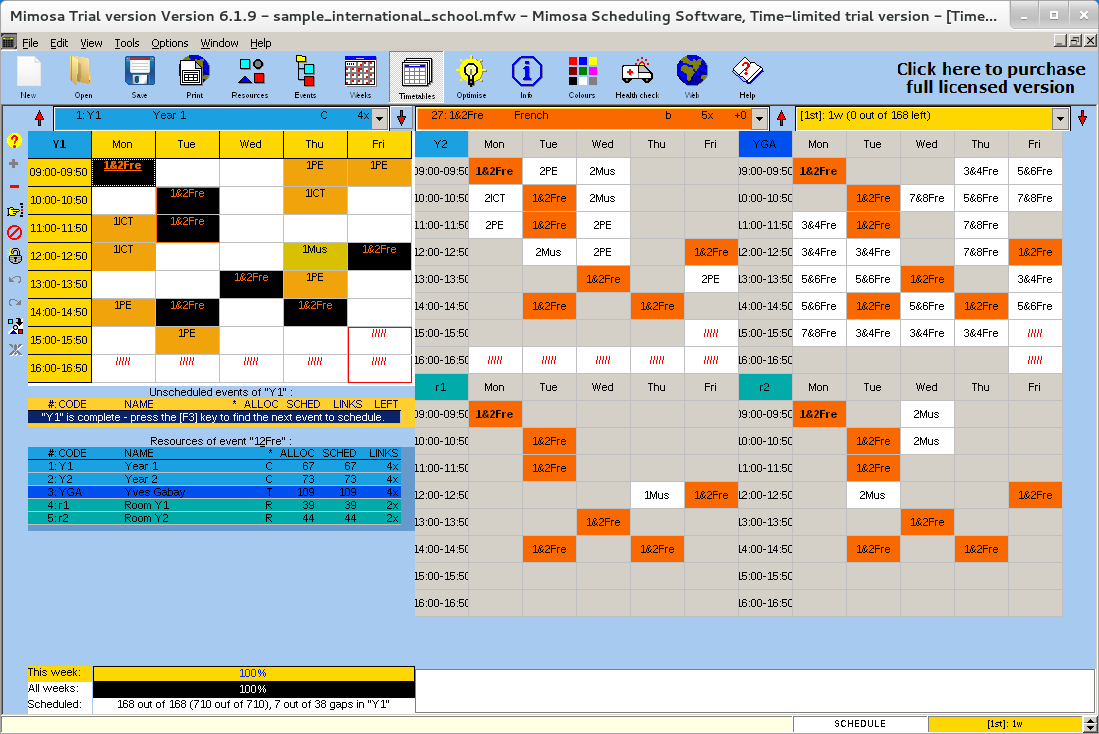
\includegraphics[width=15cm]{img/mimosa.png}
\caption{Zrzut ekranu z widoku planu zajęć programu Mimosa}
\end{figure}
\subsection{FET - Free Evolutionary Timetable}
Jest to program darmowy, stworzony dla platformy Linux, rozpowszechniany na zasadach licencji GNU GPL. Napisany w C++ z wykorzystaniem biblioteki Qt, dane pobiera z plików w formacie XML. W swojej początkowej formie opierał się na algorytmie genetycznym, który jednak poczynając od wersji 5.0.0 wydanej w 2007 roku został zastąpiony autorską heurystyką nazwaną przez autora \emph{rekursywnym zamienianiem}. Naśladuje on proces manualnego układania planu zajęć i okazał się dużo szybszy i wydajniejszy dla złożonych problem w porównaniu ze swoim poprzednikiem. Jego rozbudowany interfejs umożliwia śledzenie procesu ewolucji najlepszego rozwiązania.
\subsection{Tablix}
Jest to polski produkt typu \emph{open source}, jego autorem jest Tomasz Solc. Program powstał w technologii języka C z użyciem pakietu PVM, który umożliwia zrównoleglenie obliczeń, co znacząco przyspiesza działanie algorytmu. Dane wejściowe muszą znajdować się w plikach XML. Głównym mechanizmem, na którym opiera się program jest zrównoleglony algorytm genetyczny. Zastosowania stworzonego jądra systemu mogą dotyczyć najróżniejszych problemów optymalizacyjnych, lecz w swojej pierwotnej implementacji zostało przystosowane do problemu układania planu zajęć. Nie posiada natomiast interfejsu graficznego, który umożliwiałby edycję danych lub wizualizację wyników.
